\NeedsTeXFormat{LaTeX2e}
\documentclass[12pt,oneside,a4paper]{article}
\usepackage[left=2cm, right=2cm, top=1cm, bottom=2cm]{geometry}
\usepackage{amsmath,amsfonts,amssymb,amsthm}
\usepackage[utf8]{vietnam}
\usepackage{graphicx}
\usepackage{float}
\usepackage{mathptmx}
\usepackage{multicol}
\usepackage{enumitem} 
\usepackage{tasks} 
\usepackage{booktabs}
\usepackage{caption}
\usepackage{hyperref}

\everymath{\displaystyle}
\theoremstyle{definition}
\newtheorem{bt}{} 
\renewcommand{\thebt}{\textbf{\large Q\arabic{bt}}} 

\newcommand{\bb}[1]{\mathbb{#1}}

\newlist{questions}{enumerate}{1}
\setlist[questions]{label=\textbf{Q$_{\mathbf{\arabic*}}$:}, leftmargin=4em}

\settasks{label=\textbf{\Alph*.}, label-width=1.5em, item-indent=7mm}

\begin{document}
	\renewcommand{\figurename}{Figure}
	\renewcommand{\tablename}{Table}
	
	\begin{center}
		\textbf{\Large EXPERIMENT 3}
		
		\vspace{0.5cm}
		\textbf{{\Large INDUCTOR AND FREE OSCILLATIONS IN RLC CIRCUIT}}
	\end{center}
	
	\vspace{0.5cm}
	
	\noindent
	\begin{minipage}[t]{0.5\textwidth}
		\vspace{0.5cm}
		\textbf{Class: IT-E10 02} \\[0.2cm]
		\textbf{Group: 3} \\[0.2cm]
		\textbf{Name: Nguyễn Trọng Phúc Anh} \\[0.2cm]
		\textbf{Student ID: 202516522}
	\end{minipage}%
	\begin{minipage}[t]{0.5\textwidth}
		\vspace{0pt}
		\centering
		\textit{\textbf{Verification of the instructors}} \\[0.2cm]
		\begin{tabular}{|p{3.5cm}|p{3.5cm}|}
			\hline
			& \\[2.5cm]
			\hline
		\end{tabular}
	\end{minipage}
	
	\vspace{0.8cm}
	
	\section*{1.THEORETICAL BACKGROUND}
	
	\subsection*{1.1. Inductor and RL circuit}
	An inductor is a 2-terminal circuit element that stores energy in its magnetic field. If a current $i(t)$ is flowing through an inductor, the voltage $V_L$ across the inductor is proportional to the time rate of change of $i$:
	\begin{equation}
		V_L = L \frac{di(t)}{dt}
	\end{equation}
	where $L$ is the inductance in Henry (H).
	When a wound coil is connected with a voltage source $V_S$, we can consider it a series RL circuit. Applying Kirchhoff's voltage law:
	\begin{equation}
		V_S = V_L + V_R = L \frac{di(t)}{dt} + i(t) R = 0
	\end{equation}
	When the voltage source is replaced with a short-circuit, the current in the circuit decays exponentially with time constant $\tau = \frac{L}{R}$:
	\begin{equation}
		i(t) = I_0 e^{-\frac{t}{\tau}}
	\end{equation}
	where $I_0 = \frac{V_S}{R}$ is the current through the circuit at time $t=0$, and $R$ is the pure resistance of the coil:
	\begin{equation}
		R = \frac{V_S}{I_0}
	\end{equation}
	Taking the natural logarithm of both sides of Eq. (3):
	\begin{equation}
		\ln i(t) = -\frac{R}{L}t + \ln I_0
	\end{equation}
	Eq. (5) is a linear function of time $t$ of which the graph has the slope $S = -\frac{R}{L}$. Therefore, the inductance $L$ can be calculated as:
	\begin{equation}
		L = \frac{R}{|S|} = \frac{V_S}{I_0 \cdot |S|}
	\end{equation}
	\begin{center}
		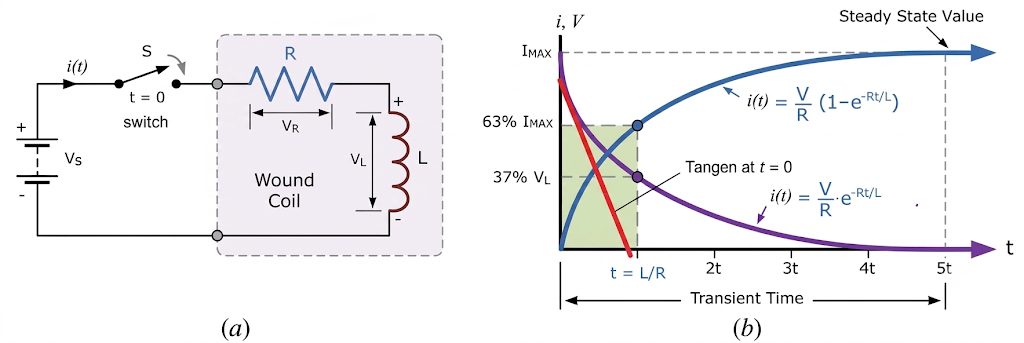
\includegraphics[width= \textwidth]{Log Graph}
		\captionof{figure}{\textit{Principal RL circuit (a) and currents flow through the circuit (b)}}
	\end{center}
	
	\subsection*{1.2. Oscillation in RLC circuit}
	For a series LC circuit where the internal resistance of the inductor is non-negligible, it can be considered an RLC circuit. The differential equation without any external voltage is:
	\begin{equation}
		L \frac{d^2 i}{dt^2} + R \frac{di}{dt} + \frac{i}{C} = 0
	\end{equation}
	The solution of Eq. (7) is:
	\begin{equation}
		i(t) = I_0 e^{-\gamma t} \cos(\omega t)
	\end{equation}
	where the exponential decay coefficient $\gamma = \frac{R}{2L}$, and the natural angular frequency of the LC oscillator is $\omega^2 = \frac{1}{LC}$ $\left( \text{or we can say } \omega = \dfrac{1}{\sqrt{LC}} \right)$.
	\begin{center}
	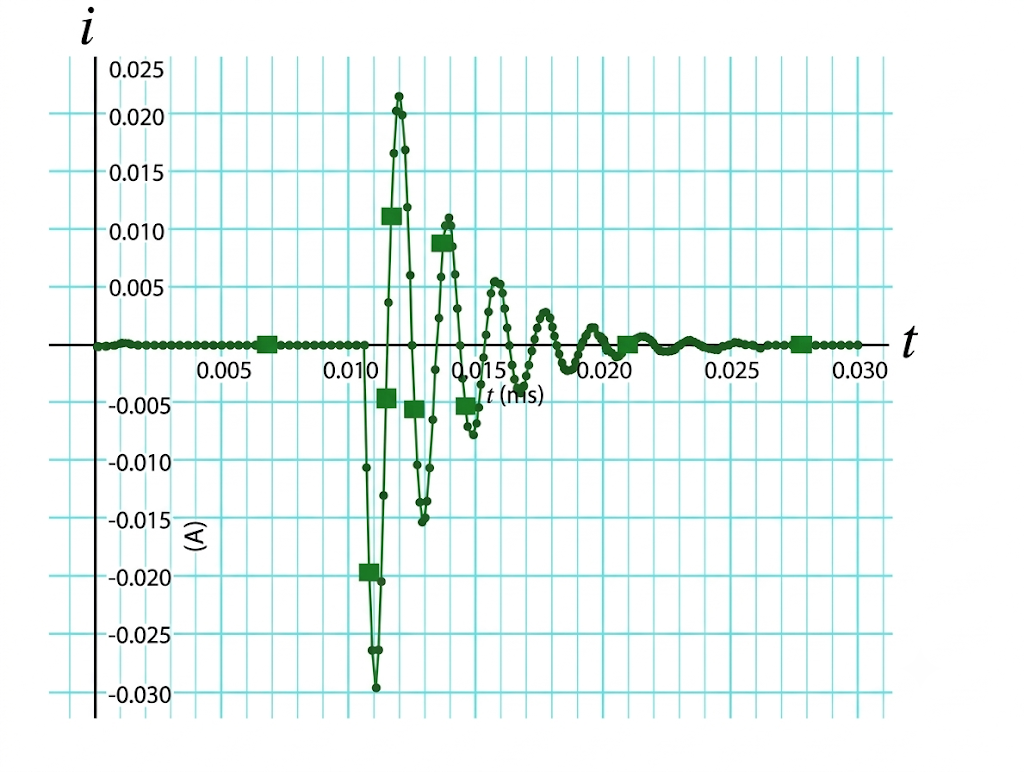
\includegraphics[width= 0.9\textwidth]{RLC circuit graph}
	\captionof{figure}{\textit{Current in a RLC circuit}}
	\end{center}
	
	\subsection*{1.3. Energy in RLC circuit}
	The energy stored in the magnetic field of the inductor is:
	\begin{equation}
		U_B = \frac{1}{2} L i^2
	\end{equation}
	and in the electric field of the capacitor is:
	\begin{equation}
		U_E = \frac{1}{2} C V^2
	\end{equation}
	The total energy stored in the electric and magnetic fields is:
	\begin{equation}
		U = U_B + U_E = \frac{1}{2} L i^2 + \frac{1}{2} C V^2
	\end{equation}
	This energy is gradually being lost as heat in the resistor at the rate $I^2 R$ (Joule heating).
		\begin{center}
		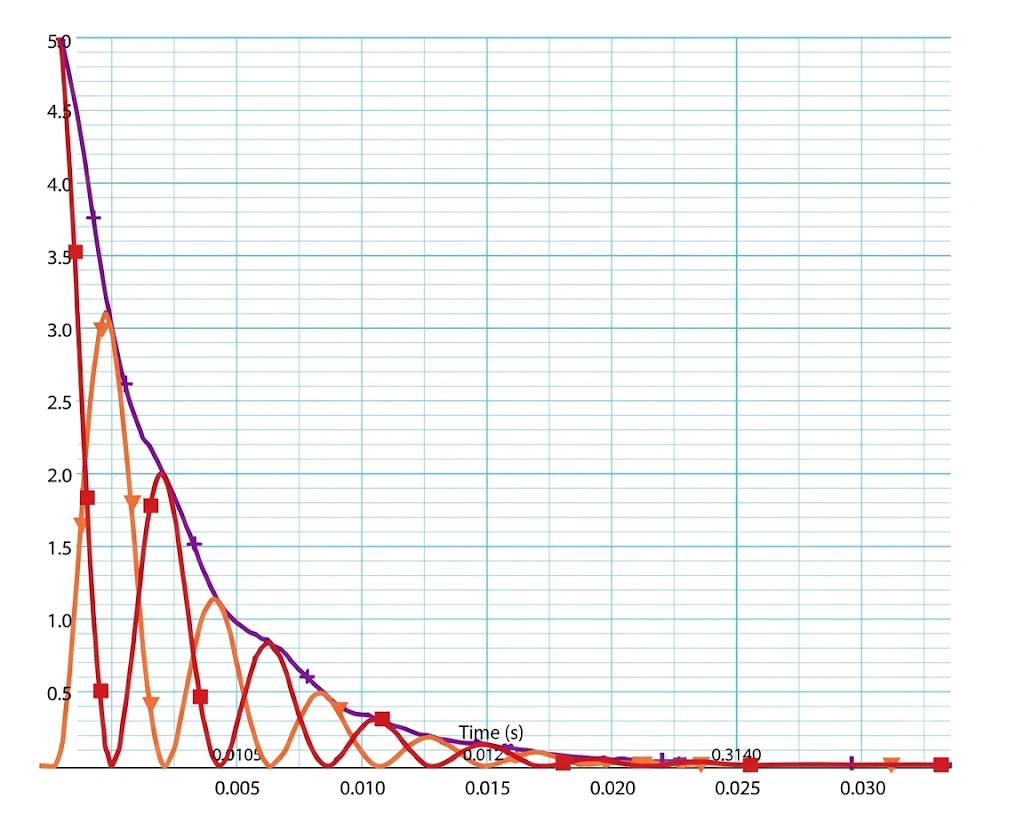
\includegraphics[width= \textwidth]{Energy in RLC}
		\captionof{figure}{\textit{Energy in RLC circuit also exponential decays}}
	\end{center}
	
	\section*{2. EXPERIMENTAL PROCEDURE}
	
	\subsection*{2.1. Current, resistance and inductance in RL circuit}
	\subsubsection*{2.1.1. Preparation for measurement}
	\begin{itemize}[leftmargin=1.5em]
		\item Connect two terminals of the coil to the springs next to the top banana jack. Connect patch cords from "OUTPUT" ports of interface to banana jacks on the board.
		\item Set up Data Studio: Connect Voltage Sensor to Channel A, Power Amplifier to Channel C.
		\item Set Signal Generator: Positive Square Wave, frequency 20 Hz, Amplitude 1 V, Sample rate 10,000 Hz, measurement time 0.5 s.
	\end{itemize}
	
	\subsubsection*{2.1.2. Measurement sequence}
	\begin{enumerate}[leftmargin=1.5em]
		\item Click "Start". Drag $\text{Run}^\#1$ file to "Graph" to display output voltage. Define and record $I_0$. Calculate coil resistance $R$ using $R = \frac{V_S}{I_0}$ with $V_S = 1\text{ V}$.
		\item Click "Calculate", apply $\ln$ function to measurement data according to Eq. (5).
		\item Drag the calculated $\ln i(t)$ result to graph display. Select linear region and perform "Curve Fit / Linear Fit" to obtain the Slope ($S$).
		\item Calculate inductance $L$ using $L = \frac{V_S}{I_0 \cdot S}$.
		\item Insert a metal core inside the coil and repeat Steps 1 to 4 to determine inductance with core.
	\end{enumerate}
	
	\subsection*{2.2. Current and energy in RLC circuit}
	\subsubsection*{2.2.1 Preparation for measurement}
	\begin{itemize}[leftmargin=1.5em]
		\item Connect a $10\,\mu\text{F}$ capacitor in series with the coil. Connect Voltage Sensor across capacitor terminals.
		\item Keep the measurement regime established in Section 2.1.1.
	\end{itemize}
	
	\subsubsection*{2.2.2 Measurement sequence}
	\begin{enumerate}[leftmargin=1.5em]
		\item Click "Start" to record data.
		\item Calculate magnetic energy $U_B = \frac{1}{2} L i^2$ using "pow(x,2)" function with calculated $L$ (without core).
		\item Calculate electric energy $U_E = \frac{1}{2} C V^2$ using $C = 10\,\mu\text{F} = 0.00001\text{ F}$.
		\item Calculate total energy $U = U_B + U_E$.
		\item Display graphs of $U_B$, $U_E$, and total energy $U$.
		\item Save all data to storage.
	\end{enumerate}
	
	\section*{3. EXPERIMENTAL RESULTS}
	\subsection*{3.1. Resistance and Inductance of the Coil}
	\hspace{1.23em}
	Initial current $\text{ I}_0 = 0.13 \text{ A}$
	
	\vspace{0.2cm}
	Measured slope (without core) $\text{S}_{\text{w/o}} = -951.50$
	
	\vspace{0.2cm}
	Measured slope (without core) $\text{S}_{\text{w}} = -190.35$
	
	\vspace{0.2cm}
	The resistance of the coil
	\begin{center}
	\fbox{%
		\begin{minipage}{0.8\textwidth}
			\vspace{-0.4cm}
			\centering
			\begin{displaymath}
				R_L = \frac{V_S}{I_0} = \dfrac{1}{0.13} \approx 7.69 \left(\Omega\right)
			\end{displaymath}
		\end{minipage}%
	}
	\end{center}
	
	Coil inductance without core
	\begin{center}
		\fbox{%
			\begin{minipage}{0.8\textwidth}
				\vspace{-0.4cm}
				\centering
				\begin{displaymath}
					L_{\text{w/o}} = \dfrac{V_S}{I_0  \left|\text{S}_{\text{w/o}}\right|} \approx \dfrac{1}{0.13 \times 951.50} \approx 8.10 \times 10^{-3}  \left(\text{H}\right) = 8.10 \left(\text{mH}\right)
				\end{displaymath}
			\end{minipage}%
		}
	\end{center}
		
	Coil inductance with core
	\begin{center}
		\fbox{%
			\begin{minipage}{0.8\textwidth}
				\vspace{-0.4cm}
				\centering
				\begin{displaymath}
					L_{\text{w}} = \dfrac{V_S}{I_0  \left|\text{S}_{\text{w}}\right|} \approx \dfrac{1}{0.13 \times 190.35} \approx 40.41 \times 10^{-3}  \left(\text{H}\right) = 40.41 \left(\text{mH}\right)
				\end{displaymath}
			\end{minipage}%
		}
	\end{center} 
	
	\begin{bt}
		\textit{Briefly explain the difference of inductance of the coil (with/without core)}
	\end{bt}
	After placing an iron core inside the coil, the coil's inductance increases. This phenomenon occurs since iron has a high magnetic permeability compared to air, enhancing the magnetic flux linkage per unit current inside the coil.
	
	\subsection*{3.2. Free Oscillations of the RLC circuit}
	\hspace{1.23em}
	Measured period $\text{ T}_{\text{measured}} = 0.0017 \text{ s}$
	
	\vspace{0.2cm}
	Measured frequency
	\begin{center}
		\fbox{%
			\begin{minipage}{0.8\textwidth}
				\vspace{-0.4cm}
				\centering
				\begin{displaymath}
					\text{f}_{\text{measured}} = \dfrac{1}{\text{T}_{\text{measured}}} = \dfrac{1}{0.0017} \approx 588.24 \left(\text{Hz}\right)
				\end{displaymath}
			\end{minipage}%
		}
	\end{center}
	
	Expected frequency (theoretical frequency)
	\begin{center}
		\fbox{%
			\begin{minipage}{0.8\textwidth}
				\vspace{-0.4cm}
				\centering
				\begin{displaymath}
					\text{f}_{\text{prediction}} = \dfrac{1}{2\pi \sqrt{L_{\text{w/o}} C}} \approx \dfrac{1}{2\pi\sqrt{\left(8.10 \times 10^{-3}\right) \times \left(10 \times 10^{-6}\right)}} \approx 559.21 \left(\text{Hz}\right)
				\end{displaymath}
			\end{minipage}%
		}
	\end{center}
	
	Frequency difference
	\begin{center}
		\fbox{%
			\begin{minipage}{0.8\textwidth}
				\vspace{-0.4cm}
				\centering
				\begin{displaymath}
					\Delta \text{f} = \text{f}_{\text{prediction}} - \text{f}_{\text{measured}} = 559.21 - 588.24 = -29.03 \left(\text{Hz}\right)
				\end{displaymath}
			\end{minipage}%
		}
	\end{center}
	
	\begin{bt}
		\textit{Comments and conclusions on frequency comparison ($\text{f}_{\text{prediction}}$ vs $\text{f}_{\text{measured}}$)}
		
		\vspace{0.2cm}
		The measured frequency ($\text{f}_{\text{measured}} \approx 588.24\text{ Hz}$) is higher than the theoretical prediction ($\text{f}_{\text{prediction}} \approx 559.21\text{ Hz}$), with an absolute difference of $\left|\Delta \text{f}\right| = 29.03\text{ Hz}$.   This discrepancy primarily comes from the non-ideal properties of the circuit components, including the internal resistance and inductance of the connecting wires, as well as the uncertainty in the nominal values of $L$ and $C$. Overall, the measured result shows reasonable agreement with the theoretical model for free RLC oscillations.
	\end{bt}
	
	\begin{bt}
		\textit{Make the comment and discussions of obtained result of energy in RLC circuit. It can be seen that the circuit is losing energy most rapidly at times when the graph of total energy is steepest; these times occur at about the same times that the magnetic energy reaches a local maximum. Briefly explain why.}
		\subsubsection*{1. Comment}
		\hspace{1.23em}
		After the external power source is disconnected, the total energy of the circuit does not drop instantly to zero; instead, it decays gradually. Energy continuously shifts back and forth between the capacitor's electric field and the inductor's magnetic field in a damped cycle, with peak levels decline over time.
		
		\vspace{0.2cm}
		
		\subsubsection*{2. Explanation}
		\hspace{1.23em}
		By the Eq. $(11)$, take derivatives in both sides, notice that $U_E = \dfrac{1}{2} CV^2 = \dfrac{1}{2} \dfrac{q^2}{C}$
		\begin{equation}
			\dfrac{dU}{dt} = \dfrac{dU_B}{dt} + \dfrac{dU_E}{dt} = iL \dfrac{di}{dt} + q\dfrac{dq}{dt} \dfrac{1}{C} = iL \dfrac{di}{dt} + q \dfrac{i}{C} = i\left(L\dfrac{di}{dt} + \dfrac{q}{C}\right)
		\end{equation}
		
		By Kirchoff's law for RLC circuit, we have
		\begin{equation}
			V_L + V_S + V_C = 0 \implies L\dfrac{di}{dt} + iR + \dfrac{q}{C} = 0 \implies -iR = L\dfrac{di}{dt} + \dfrac{q}{C} \implies \dfrac{dU}{dt} = -i^2R
		\end{equation}
		
		Hence, the total energy in a damped RLC circuit decreases over time due to Joule heating across the resistor, with a rate of energy loss given by $\frac{dU}{dt} = -i^2 R$. The circuit loses energy most rapidly when the absolute rate of energy change (the slope of the total energy curve) is at its maximum, which occurs precisely when the magnitude of the current $\vert{}i\vert{}$ reaches its peak. Since the magnetic energy stored in the inductor is expressed as $U_B = \frac{1}{2} L i^2$, these peak current moments correspond directly to the local maxima of the magnetic energy. Consequently, the steepest points on the total energy graph coincide with the times when magnetic energy reaches its local maximum.
	\end{bt}
	
\end{document}